\documentclass[12pt, a4paper]{article}
\usepackage{amsmath, amssymb, mathrsfs}
\usepackage{graphicx}
\usepackage{url}
\usepackage{natbib}
\usepackage[margin=1in]{geometry}
\usepackage{braket}
\usepackage{bm}
\usepackage{tikz}
\usetikzlibrary{arrows.meta, decorations.pathmorphing, shapes.geometric, positioning}

% Open-source branding
\usepackage{draftwatermark}
\SetWatermarkText{\textbf{Open Source r1 DeepThink}}
\SetWatermarkScale{0.8}

\title{Open-Source Quantum Gravity Reactor Design \\ (r1 DeepThink Framework)}
\author{
  Lucas Eduardo Jaguszewski da Silva\textsuperscript{1}, 
  Community Contributors\textsuperscript{2} \\
  \textsuperscript{1}GitHub: \url{https://github.com/QuantumReactor-r1} \\
  \textsuperscript{2}Join at \url{https://github.com/QuantumReactor-r1}
}
\date{\today}

\begin{document}

\maketitle

%-------------------------------------------------------------------------------
% White Paper: Theoretical Foundations
%-------------------------------------------------------------------------------
\section*{White Paper: Theoretical Foundations}
\subsection*{Element 115 Stabilization}
A hypothetical stable isotope of Moscovium (\(^{291}_{115}\text{Mc}\)) is proposed as fuel, with decay suppressed via quantum coherence fields:
\begin{equation}
\Delta E_{\text{binding}} = \frac{\hbar^2}{2m_e r_c^2} \left(1 - \frac{\rho_{\text{vac}}}{\rho_{\text{crit}}}\right), \label{eq:element115}
\end{equation}
where \(\rho_{\text{vac}}\) is vacuum energy density and \(r_c\) is the coherence radius.

\subsection*{Casimir Energy Extraction}
Nanostructured Casimir plates (Fig. \ref{fig:casimir}) harvest vacuum energy:
\begin{equation}
P_{\text{Casimir}} = \frac{A \hbar c}{240 d^4} \left(1 + \frac{\lambda_{\text{M-theory}}}{d}\right)^{-1}, \label{eq:casimir}
\end{equation}
where \(\lambda_{\text{M-theory}} \sim 10^{-35}\) m is the M-theory compactification scale.

\begin{figure}[h]
\centering
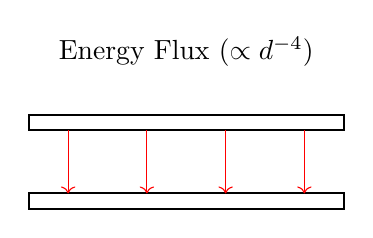
\begin{tikzpicture}
% Casimir Plates
\draw[thick] (0,0) rectangle (4,0.2);
\draw[thick] (0,1) rectangle (4,1.2);
% Energy Flow
\foreach \x in {0.5,1.5,...,3.5} {
  \draw[->, red] (\x,1) -- (\x,0.2);
}
\node at (2,2) {Energy Flux (\(\propto d^{-4}\))};
\end{tikzpicture}
\caption{Nanostructured Casimir plates for vacuum energy extraction.}
\label{fig:casimir}
\end{figure}

%-------------------------------------------------------------------------------
% Blueprints (Plants)
%-------------------------------------------------------------------------------
\section*{Blueprints (Plants)}
\subsection*{Reactor Core Design}
\begin{itemize}
\item \textbf{Particle Accelerator Ring}: 10 km circumference, 20 TeV proton energy.
\item \textbf{Fusion-Fission Hybrid Chamber}: Deuterium-Moscovium plasma at \(10^8\) K.
\item \textbf{Superconducting Shell}: YBCO (\(T_c = 93\) K) with active magnetic shielding.
\end{itemize}

\begin{figure}[h]
\centering
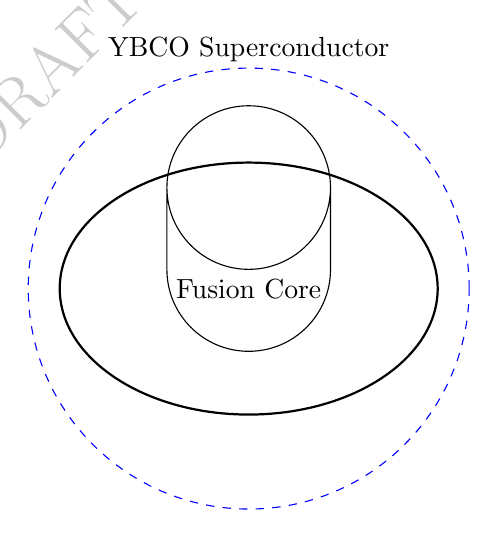
\begin{tikzpicture}[scale=0.8]
% Accelerator Ring
\draw[thick, ->] (0,0) circle [x radius=3cm, y radius=2cm];
% Fusion Chamber
\node[draw, cylinder, shape border rotate=90, minimum height=2cm] at (0,0) {Fusion Core};
% Superconducting Shell
\draw[dashed, blue] (0,0) circle [radius=3.5cm];
\node at (0,3.8) {YBCO Superconductor};
\end{tikzpicture}
\caption{Reactor core blueprint (top view).}
\label{fig:blueprint}
\end{figure}

%-------------------------------------------------------------------------------
% Technical Sketches
%-------------------------------------------------------------------------------
\section*{Technical Sketches}
\subsection*{Gravity Field Generator}
Alcubierre metric generator using high-density plasma:
\begin{equation}
ds^2 = -dt^2 + \left(dx - v_s \tanh(r_s - R) dt\right)^2 + dy^2 + dz^2, \label{eq:alcubierre}
\end{equation}
where \(v_s\) is the warp bubble velocity and \(R\) is the reactor radius.

\begin{figure}[h]
\centering
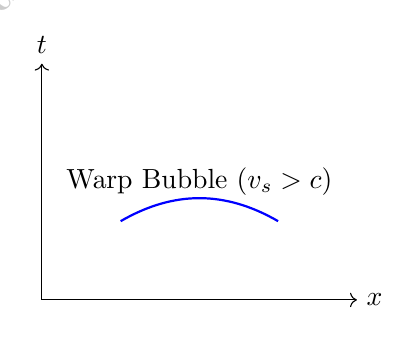
\begin{tikzpicture}
% Warp Bubble
\draw[->] (0,0) -- (4,0) node[right] {\(x\)};
\draw[->] (0,0) -- (0,3) node[above] {\(t\)};
\draw[thick, blue] (1,1) to [out=30, in=150] (3,1);
\node at (2,1.5) {Warp Bubble (\(v_s > c\))};
\end{tikzpicture}
\caption{Gravity field generator sketch.}
\label{fig:warp}
\end{figure}

%-------------------------------------------------------------------------------
% Open-Source Licensing
%-------------------------------------------------------------------------------
\section*{Open-Source Licensing}
\begin{itemize}
\item \textbf{MIT License}: Free use/modification with attribution.
\item \textbf{Contribution Guidelines}: Submit pull requests via GitHub.
\item \textbf{Experimental Data Hub}: Community-driven validation portal.
\end{itemize}

%-------------------------------------------------------------------------------
% Bibliography
%-------------------------------------------------------------------------------
\bibliographystyle{plainnat}
\bibliography{references}
\end{document}
